\begin{frame}{\acrshort{fpga} introduction}
    \begin{itemize}
        \item Field Programmable Gate Arrays
        \item Configurable Logic Block Matrix
        \item Variable granurality
        \item Dinamic and static configuration
    \end{itemize}
    \begin{figure}[!ht]
    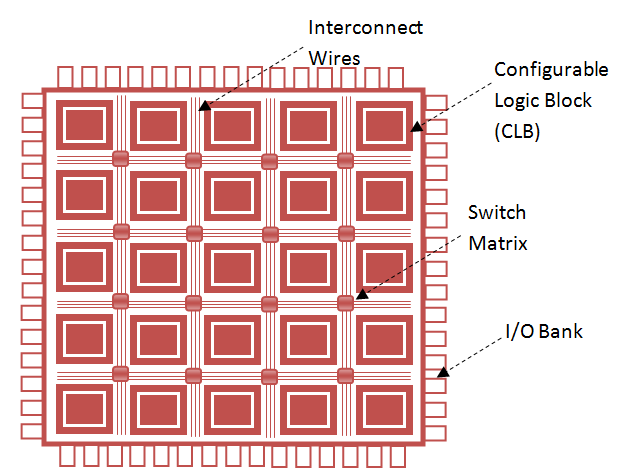
\includegraphics[width=0.5\linewidth]{images/FPGA-Architecture.png}
    \end{figure}
\end{frame}




\begin{frame}{Xilinx Spartan 7 SP701}
	\begin{columns}
    \begin{column}{0.5\textwidth} % Left column and width
	    \begin{itemize}
	    \item Chip xc7s100 serie %https://www.mouser.es/ProductDetail/?qs=unwgFEO1A6sZ6LzV7v6FSA%3D%3D
	    \begin{itemize}
	    	\item 102400 LE %Logic elements: smallest units of logic. LEs  provide advanced features with efficient logic like LUT
	   	 \item 16000 ALM %adaptive logic module: more complex boolean functions with/without registers
	    	\item 400 I/O  per second %Input output operations per second 
	    \end{itemize}
	\end{itemize}
\end{column}
\begin{column}{.5\textwidth} % Right column and width

\begin{figure}[!ht]
    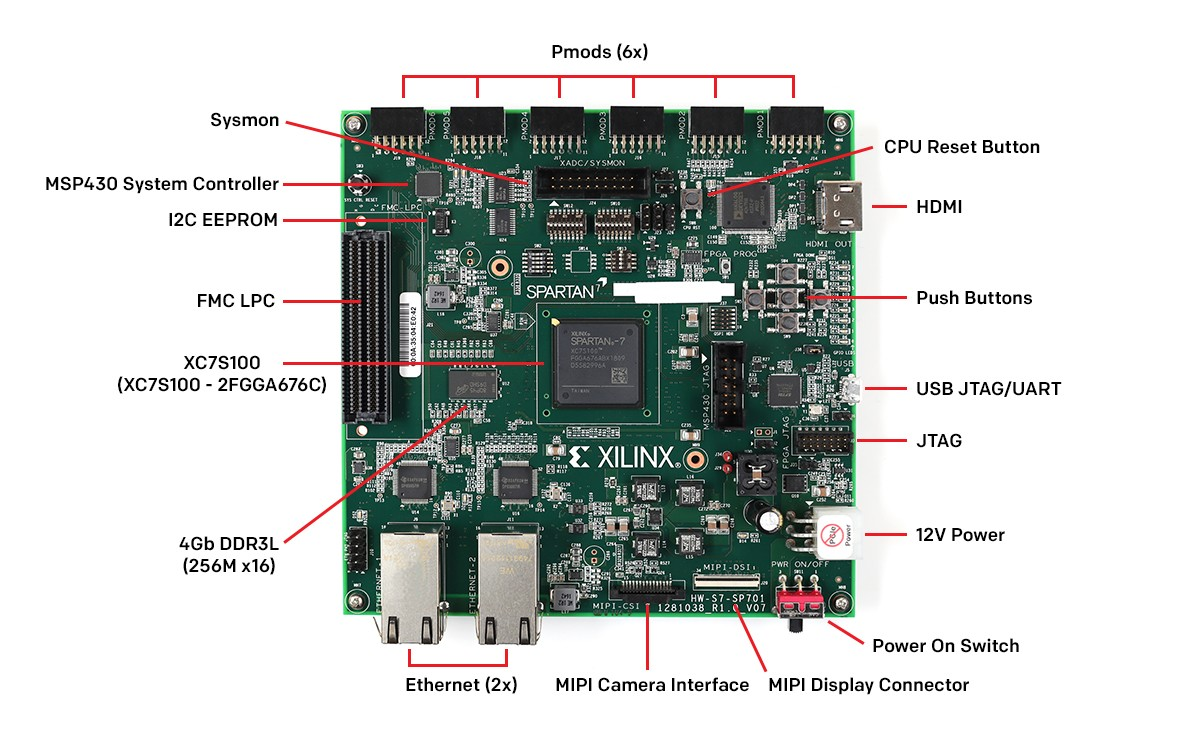
\includegraphics[width=1.3\linewidth]{images/spartan7.jpg}
\end{figure}
\end{column}
\end{columns}
\end{frame}
